\section{Ergebnisse}
Im folgenden Kapitel werden die Trainingsresultate präsentiert
Als Leistungsmaß wird die Genauigkeit, mittels Genauigkeit-Epochen-Plots
und \emph{Confusionmatrizen}, der jeweiligen Modells präsentiert.

Bei den Trainings werden die Bilder batchweise geladen und verarbeitet.
Hierbei erfolgt auch eine Normierung der Pixelwerte.
Vor dem Beginn eines Trainings werden \emph{Batch-Größe} und
\emph{Learningrate} festgelegt. Letztere wird jedoch, während des Trainings dynamisch
,durch die Funktion \textsc{ReduceLROnPlateau}, angepasst \cite{keras_ReduceLROnPlateau}.
 Die Anzahl der Trainingsepochen ist kein Hyperparameter, da hier eine \emph{EarlyStopper}
eingestetzt wird \cite{keras_EarlyStopping}.
Alle Trainingseinheiten werden auf einer \textsc{Nvidia}-Grafikkarte
durchgeführt.

\subsection{MiniDogNN--$5$ Hunderassen}
Die Hyperparameteroptimierung (HPO) variiert die Einstellung
für die $l2$-Regularisierung $l2\ua{value}$, die Batchgröße $bs$
und die Farbinformation $color$ der Bilder:
\begin{equation}
  \label{eq:Parameterraum_MiniDogNN}
  bs\in\left\{2,\, 5, \,10, \,15,\, 17,\, 25\right\}, \quad l2\ua{value}\in\left\{0.01, \,0.001,\, 0.005,\, 0.0001\right\}, \quad color\in\left\{\map{rgb}, \,\map{grey}\right\}
\end{equation}
Die maximale Größe der Batchgröße wird durch den Grafikspeicher limitiert.
Als anfängliche Lernrate wird $lr=0.001$ gewählt.
Das Ergebnis der HPO ist in Abbildung \ref{fig:Hyperraum_MiniDogNN} dargestellt,
deutlich ist der positive Einfluss der Farbinformation $color=\map{rgb}=\map{True}=1.0$
zu erkennen.
\begin{figure}
\centering
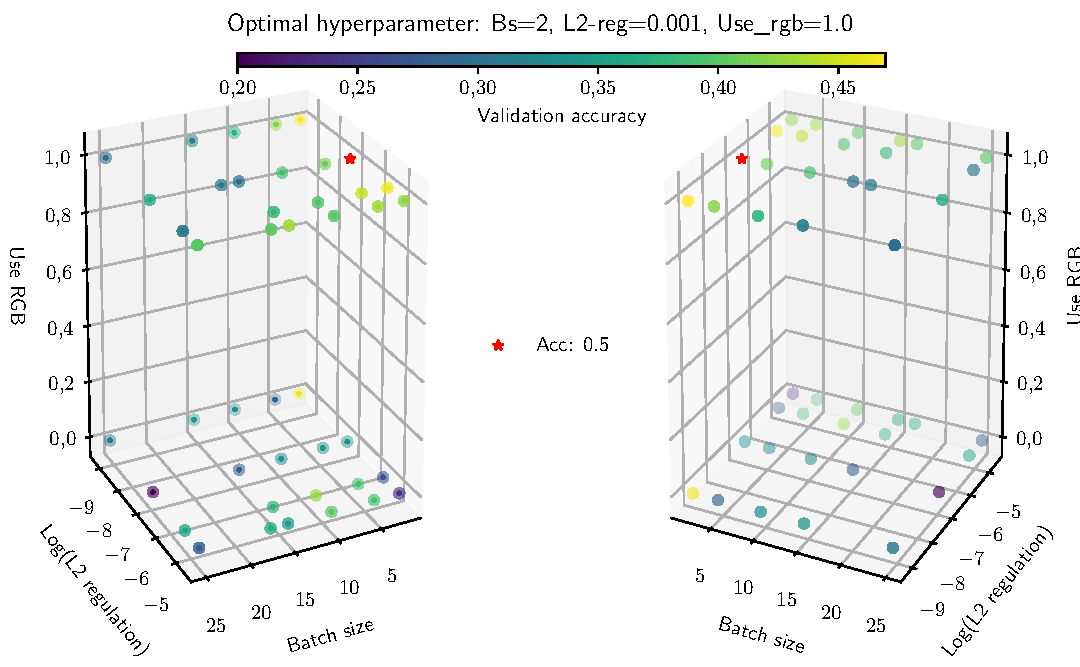
\includegraphics[width=0.5\textwidth]{../../final_data/MiniNN_n5/hyper_raum.pdf}
\caption{Ergebnis der HPO, die $z$-Achse \emph{Use RGB} gibt an, ob Farbinformation
        verwendet wurden.}
\label{fig:Hyperraum_MiniDogNN}
\end{figure}
Von den $48$ möglichen Kombinationen wurden $43$ erfolgreich beendet, die Restlichen
wurden auf Grund von Grafikspeicherproblem von \textsc{keras} abgebrochen. Eine
Genauigkeitsverteilung ist in Abbildung \ref{fig:Genauigkeitverteilung_MiniDogNN}
dargestellt. Diese verdeutlicht, dass mit HPO
eine Genauigkeitssteigerung bewirkt werden kann. Aus Zeit- und Komplexititätsgründen wird
angenommen, dass das Ergebnis der HPO, trotz anderem
FCN, sowohl auch für das $120$ Rassen \textsc{MiniDogNN} gültig ist.

In Abbildung \ref{fig:MiniDogNN_Loss_Acc} findet sich die Trainingsdokumentation,
des optimierten Modells. In dem Plot \ref{fig:MiniDogNN_Loss_Acc} ist zu erkennen,
dass die Architektur geringfügig Übertrainiert wurde.
\begin{figure}
\centering
\begin{subfigure}{0.48\textwidth}
\centering
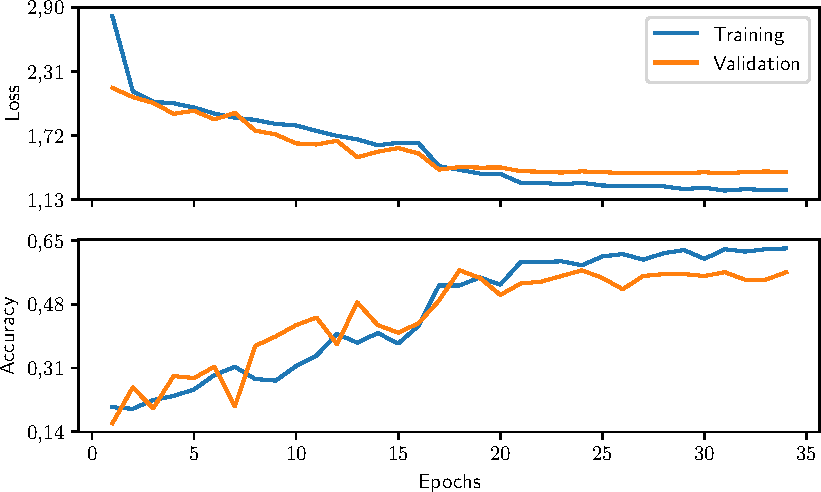
\includegraphics[width = \textwidth]{../../final_data/MiniNN_n5/history.pdf}
\caption{Trainingsfortschritt des \textsc{MiniDogNN}.}
\label{fig:MiniDogNN_Loss_Acc}
\end{subfigure}
\begin{subfigure}{0.48\textwidth}
\centering
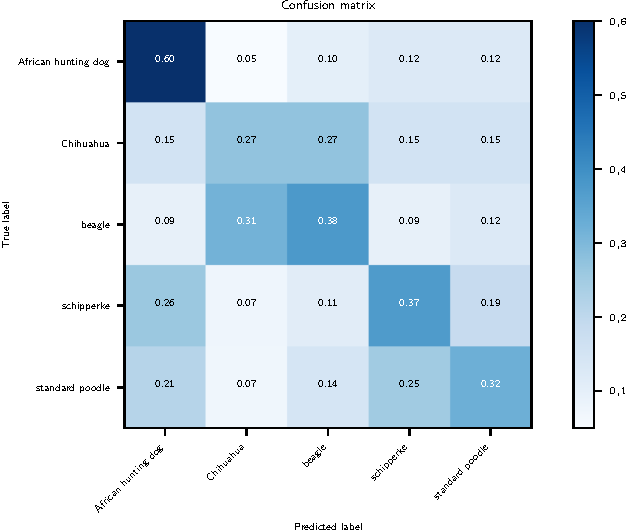
\includegraphics[width = \textwidth]{../../final_data/MiniNN_n5/confusion_matrix.pdf}
\caption{Confusionmatrix des \textsc{MiniDogNN}. Der Legendenschlüssel findet sich in
Tabelle \ref{tab:legende_rf}.}
\label{fig:MiniDogNN_Confusionmatrix}
\end{subfigure}
\caption{Traningsdokumentation \textsc{MiniDogNN}.}
\end{figure}

%\subsection{PreDogNN -- $5$ Hunderassen}
%Die \textsc{PreDogNN}-Architektur wurde mit einer Batachgröße von $16$, einer
%$l2$-Regularisierungsstärke von $l2\ua{value}=0.01$, einer Lernrate von
%$lr=0.001$, einer Dropourate von $dr=0.2$ und als Farbmodus $color=\map{rgb}$ gewählt.
%Auf Grund der Verwendung von Dropout muss der Loss und die Genauigkeit nach jeder
%Epoche berechnet werden, da sich durch Dropout die Struktur des Netzes epochenweise
%ändert. Die resultierenden Loss- und Genauigkeitverläufe befinden sich in Abbildung
%\ref{fig:PreDogNN_Loss_Acc}. Die Confusionmatrix ist in Abbildung %\ref{fig:PreDogNN_Confusionmatrix}
%dargestellt. Bemerkenswert ist die Genauigkeit der Architektur welche fast
% bei $100\%$ liegt und somit das \textsc{MiniDogNN} überbietet.
%\begin{figure}
%\centering
%\begin{subfigure}{0.48\textwidth}
%\centering
%\includegraphics[width = \textwidth]{../../final_data/PreDogNN/16-07-2019_18:39:02/build/%history_epoch.pdf}
%\caption{Trainingsfortschritt des \textsc{PreDogNN}.}
%\label{fig:PreDogNN_Loss_Acc}
%\end{subfigure}
%\begin{subfigure}{0.48\textwidth}
%\centering
%\includegraphics[width = \textwidth]{../../final_data/PreDogNN/16-07-2019_18:39:02/build/%confusion_matrix.pdf}
%\caption{Confusionmatrix des \textsc{PreDogNN}.}
%\label{fig:PreDogNN_Confusionmatrix}
%\end{subfigure}
%\end{figure}
%
\subsection{MiniDogNN -- $120$ Hunderassen}
Wie in der Abbildung \ref{fig:MiniDogNN} zu erkennen, ändert sich mit der
Anzahl der Hunderassen die Anzahl der Neuronen im FCN. Die Anzahl der generierten
Features bleibt jedoch konstant. Ein Fakt, der sich signifikant auf die
Verwendbarkeit der Architektur auswirkt. Bei dem Vergleich mit der Confusionmatrix
(vgl. Abb. \ref{fig:MiniDogNN_120_Confusionmatrix}) und
der Loss- und Genauigkeitsdokumentation (vgl. Abb. \ref{fig:MiniDogNN_120_Loss_Acc})
wir deutlich, dass die Architektur kein verwendbaren Ergebnisse liefert.

\subsection{PreBigDogNN}
Die enorme Anzahl an Features in Verbindung mit der Regularisierung ($l2\ua{value}=0.01, \, dr=0.2$)
führen dazu, dass \textsc{PreBigDogNN} eine Genauigkeit deutlich über der Rategenauigkeit
von $acc\ua{rate}=0.83\%$ erzielt. Hierbei läuft das Modell nur geringfügig in Overtraining,
wie die Trainingsdokumentation (vgl. Abb. \ref{fig:PreBigDogNN_Loss_Acc}) zeigt.
Das in der Confusionmatrix eine Diagonale ersichtlich ist, spricht für ein genaues Modell.
Jedoch ist die Genauigkeit beschränkt, was sich durch die großen Nebendiagonalelementen
äußert. Zum Beispiel wird die Rasse \emph{American Staffordshire Terrier}
in ungefährt 80 \% aller Fälle als \emph{Staffordshire Bullterrier} klassifiziert.
Wie der Name schon vermuten lässt, handelt es sich hier um Unterrassen, die
selbst wir nicht im direkten Vergleich unterscheiden können.
\begin{figure}
\centering
\begin{subfigure}{0.48\textwidth}
\centering
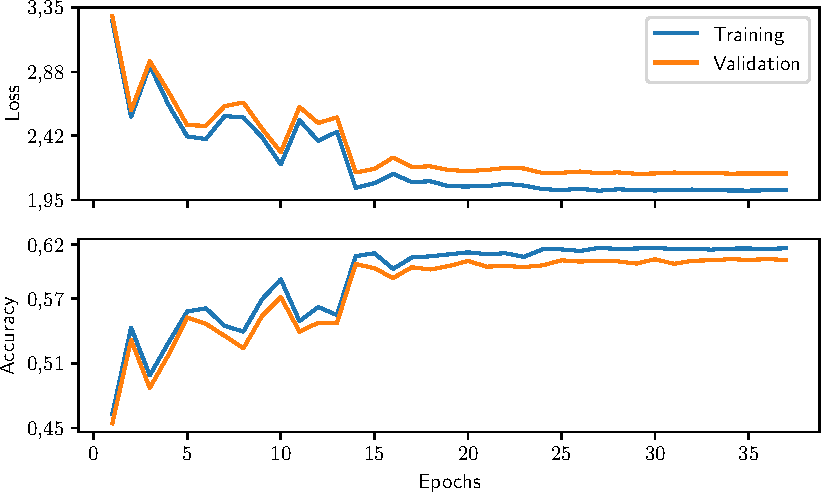
\includegraphics[width = \textwidth]{../../final_data/PreBigDogNN/17-07-2019_12:32:09/build/history_epoch.pdf}
\caption{Trainingsfortschritt des \textsc{PreBigDogNN}.}
\label{fig:PreBigDogNN_Loss_Acc}
\end{subfigure}
\begin{subfigure}{0.48\textwidth}
\centering
\includegraphics[width = \textwidth]{../../final_data/PreBigDogNN/17-07-2019_12:32:09/build/confusion_matrix.pdf}
\caption{Confusionmatrix des \textsc{PreBigDogNN}. Der Legendenschlüssel findet sich in
Tabelle \ref{tab:legende_rf}.}
\label{fig:PreBigDogNN_Confusionmatrix}
\end{subfigure}
\caption{Traningsdokumentation \textsc{PreDogNN}.}
\end{figure}
\subsection{AutoEncoder \& Randomforest}
Wie in Abbildung \ref{fig:Autoencoder} angedeutet, werden die Bilder auf eine Größe von $96\times96$ runterskaliert.
Hierdurch wird die Trainingszeit, auf Kosten der Featureanzahl,
reduziert. Analog zu den NN verwendet der Autoencoder \textsc{EarlyStopping}
und eine adaptive Lernrate. Der Autoencoder wird mit einer Batchgröße
von $bs=16$ und einer anfänglichen Lernrate von $lr=0.001$ trainiert und
erreicht eine Genauigkeit von $78\%$ (vgl. Abb. \ref{fig:Autoencoder_loss}).
Der Epochenverlauf der Losskurve (vgl. Abb. \ref{fig:Autoencoder_loss}) deutet auf Overtraining hin, was aber auf ein Skalierungsproblem der Achsen zurückzuführen ist.
Eine Tatsache, die mit der Genauigkeitsverlauf (vgl. Abb. \ref{fig:Autoencoder_loss}) untermauert werden kann.

Die Hyperparameter für den Random Forest (RF) werden zunächst mit
einer HPO für $5$ Rassen optimiert und anschließend für $120$ Rassen verwendet.
Die zu optimierenden Parameter
wurden dem Online-Guide \cite{RF_parameterraum} entnommen. Insgesamt
wird die maximale Tiefe $max_d$, die Methode zur Bestimmung der Maximalanzahl
an Bildern die pro Schnitt verwendet werden
$n\ua{feat}$, die Mindestanzahl an Bildern die einen Ast haben muss,
um berücksichtigt zu werden $min\ua{leaf}$, die Mindestanzahl an Bildern um
einen neuen Ast zu eröffnen $min\ua{split}$, das Bewertungskriterium $crit$ und
die Anzahl der Bäume $n\ua{est}$.
Eine vollständige Auflistung des Parameterraums findet sich in der
Gleichung \eqref{eq: rf_parameter_raum}.
Aus der HPO folgt für die optimale Parameterkombination:
\begin{equation*}
  max_d = 100,\,\, n\ua{feat}= log2, \,\, min\ua{leaf}= 1,\,\, min\ua{split}=10, \,\,   crit= gini, \,\, n\ua{est}=1000
\end{equation*}
\begin{wrapfigure}{r}{0.5\textwidth}
  \vspace{-25pt}
\begin{center}
\includegraphics[width=0.5\textwidth]{../../final_data/autoencoder_n_120/build/confusion_matrix.pdf}
\end{center}
\vspace{-20pt}
\caption{Confusionmatrix des Randomforest. Der Legendenschlüssel findet sich in
Tabelle \ref{tab:legende_rf}.}
\label{fig:Confusionmatrix_rf}
\vspace{-100pt}
\end{wrapfigure}
Für die Bestimmung der Genauigkeit des RF wird eine Cossvalidierung mit
drei Iterationen durchgeführt. Die HPO führt zu einer Steigerung der Genauigkeit von  $acc\ua{default, 5}=43\pm6\%$ auf $acc\ua{opt, 5}=44\pm4\%$.
Die mittlere Genauigkeit für den RF($N\ua{dr}=120$) beträgt $acc\ua{mean,120}=5\pm0.1\% > acc\ua{rate}$. Die dazugehörige Confusionmatrix ist in Abbildung \ref{fig:Confusionmatrix_rf} gezeigt.
